\chapter{資料探討}
\section{資料來源}
我們選擇了一筆2018年釋出的網路資料
\begin{itemize}
    \item \href{https://datahack.analyticsvidhya.com/contest/mckinsey-analytics-online-hackathon/}{McKinsey Analytics: Online Hackathon on Healthcare}
\end{itemize}

\section{資料基本型態}
\begin{itemize}
    \item 資料總數: 5110個人
    \item 類別型: gender, hypertension, heart\_disease, ever\_married, work\_type, Residence\_type, smoking\_status, stroke
    \item 數值型: age, avg\_glucose\_level, bmi
\end{itemize}

\section{單變數分析: 類別型}
\subsection{gender}
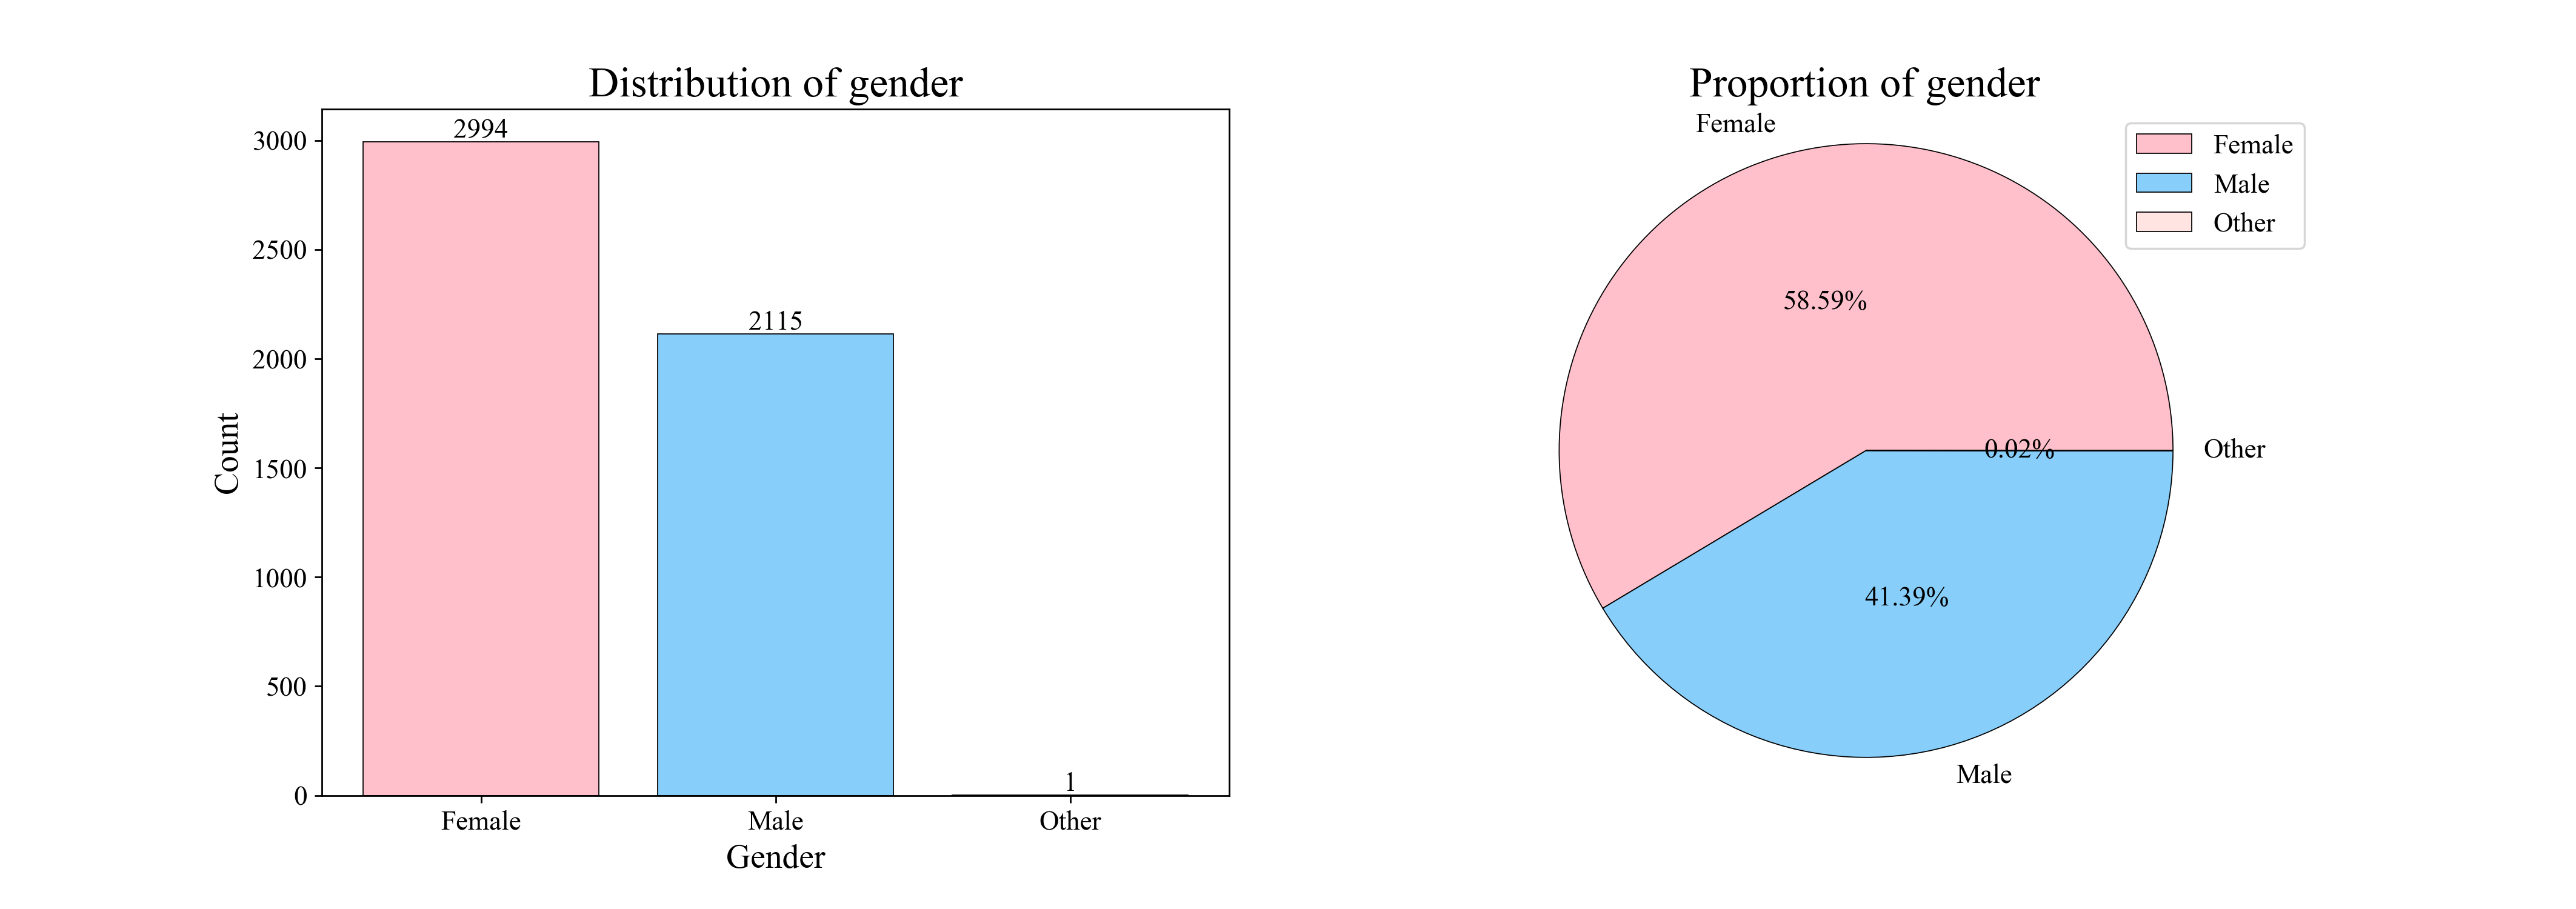
\includegraphics[width=13.5cm]{./images/gender_bar_pie.png}

\subsection{Hypertension}
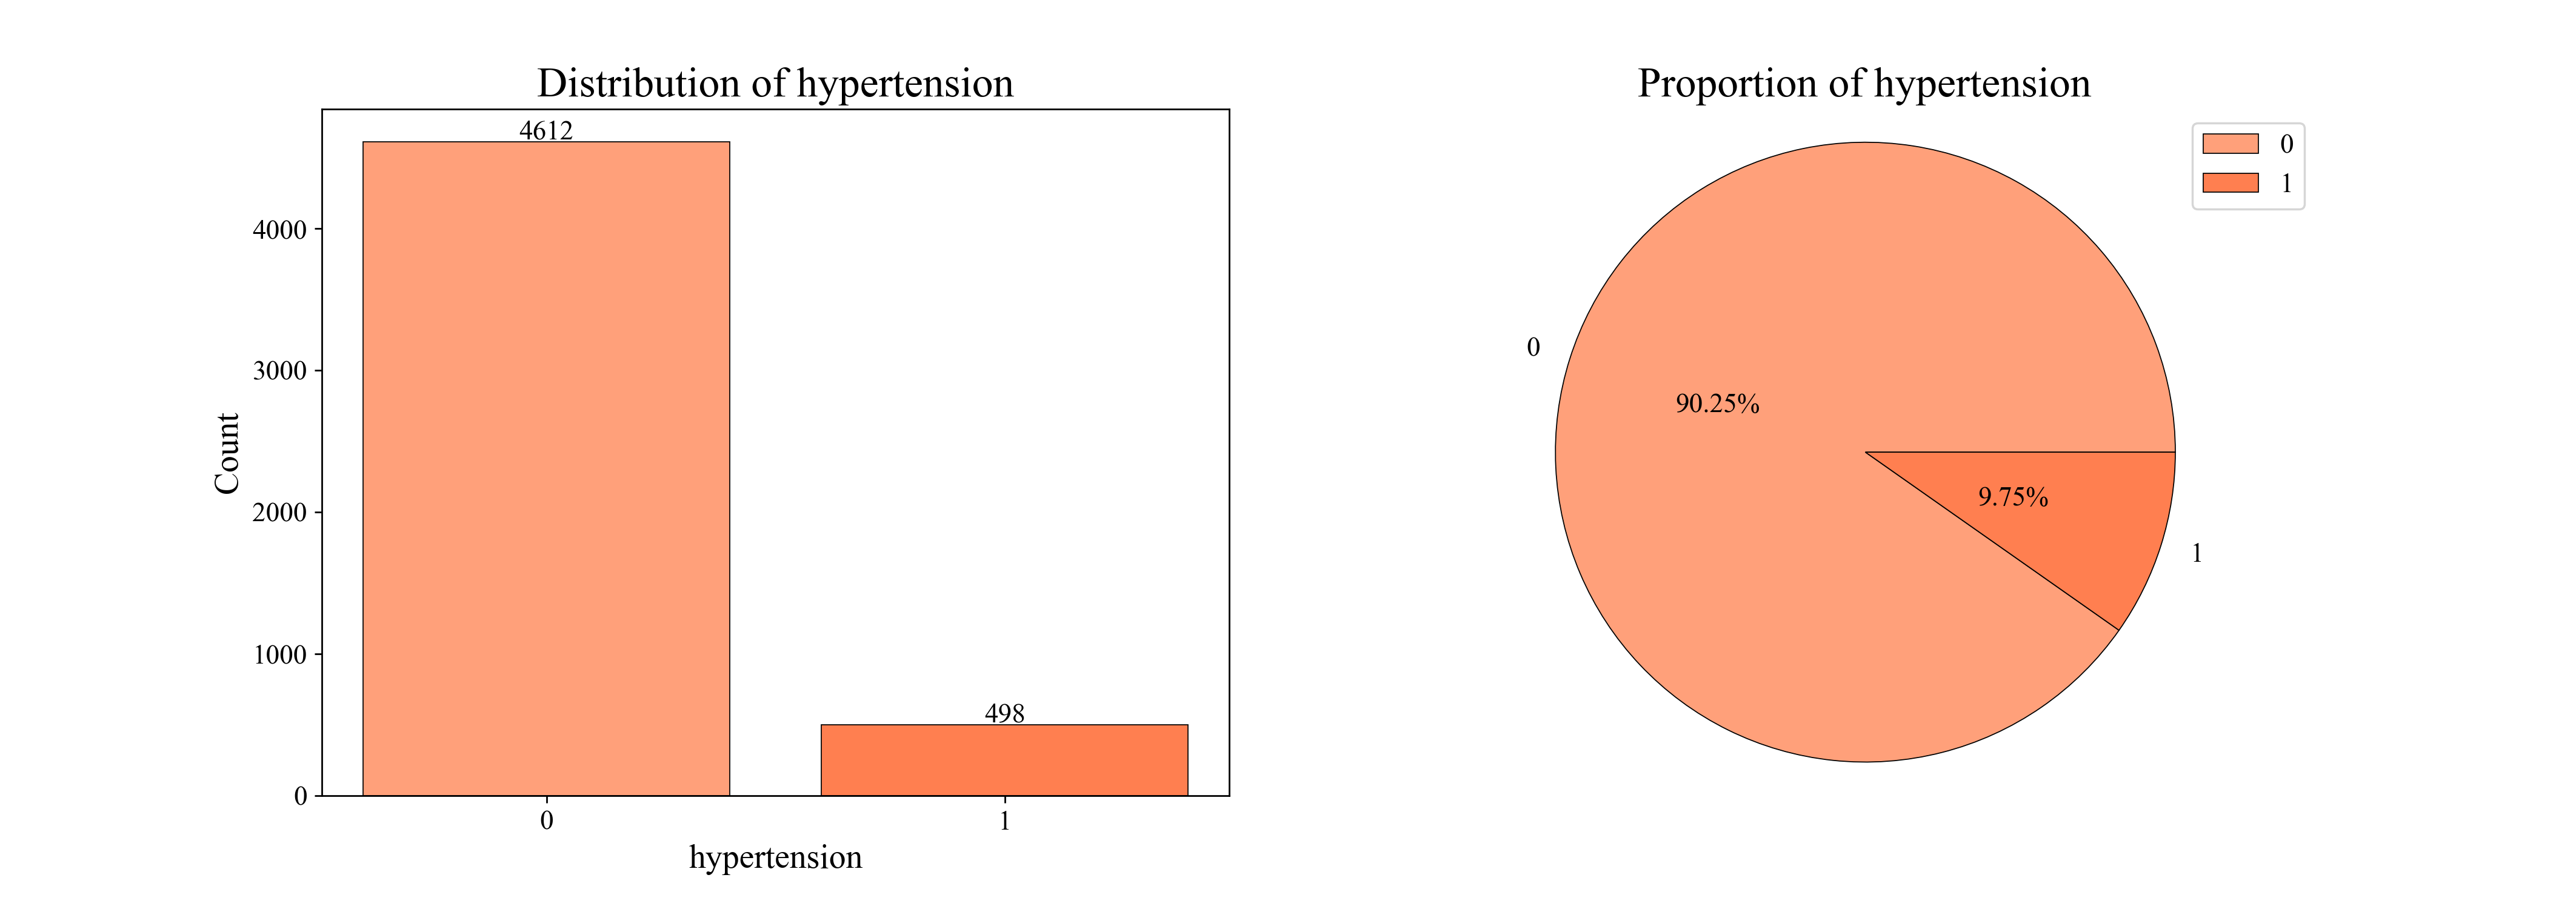
\includegraphics[width=13.5cm]{./images/hypert_bar_pie.png}

\subsection{Heart Disease}
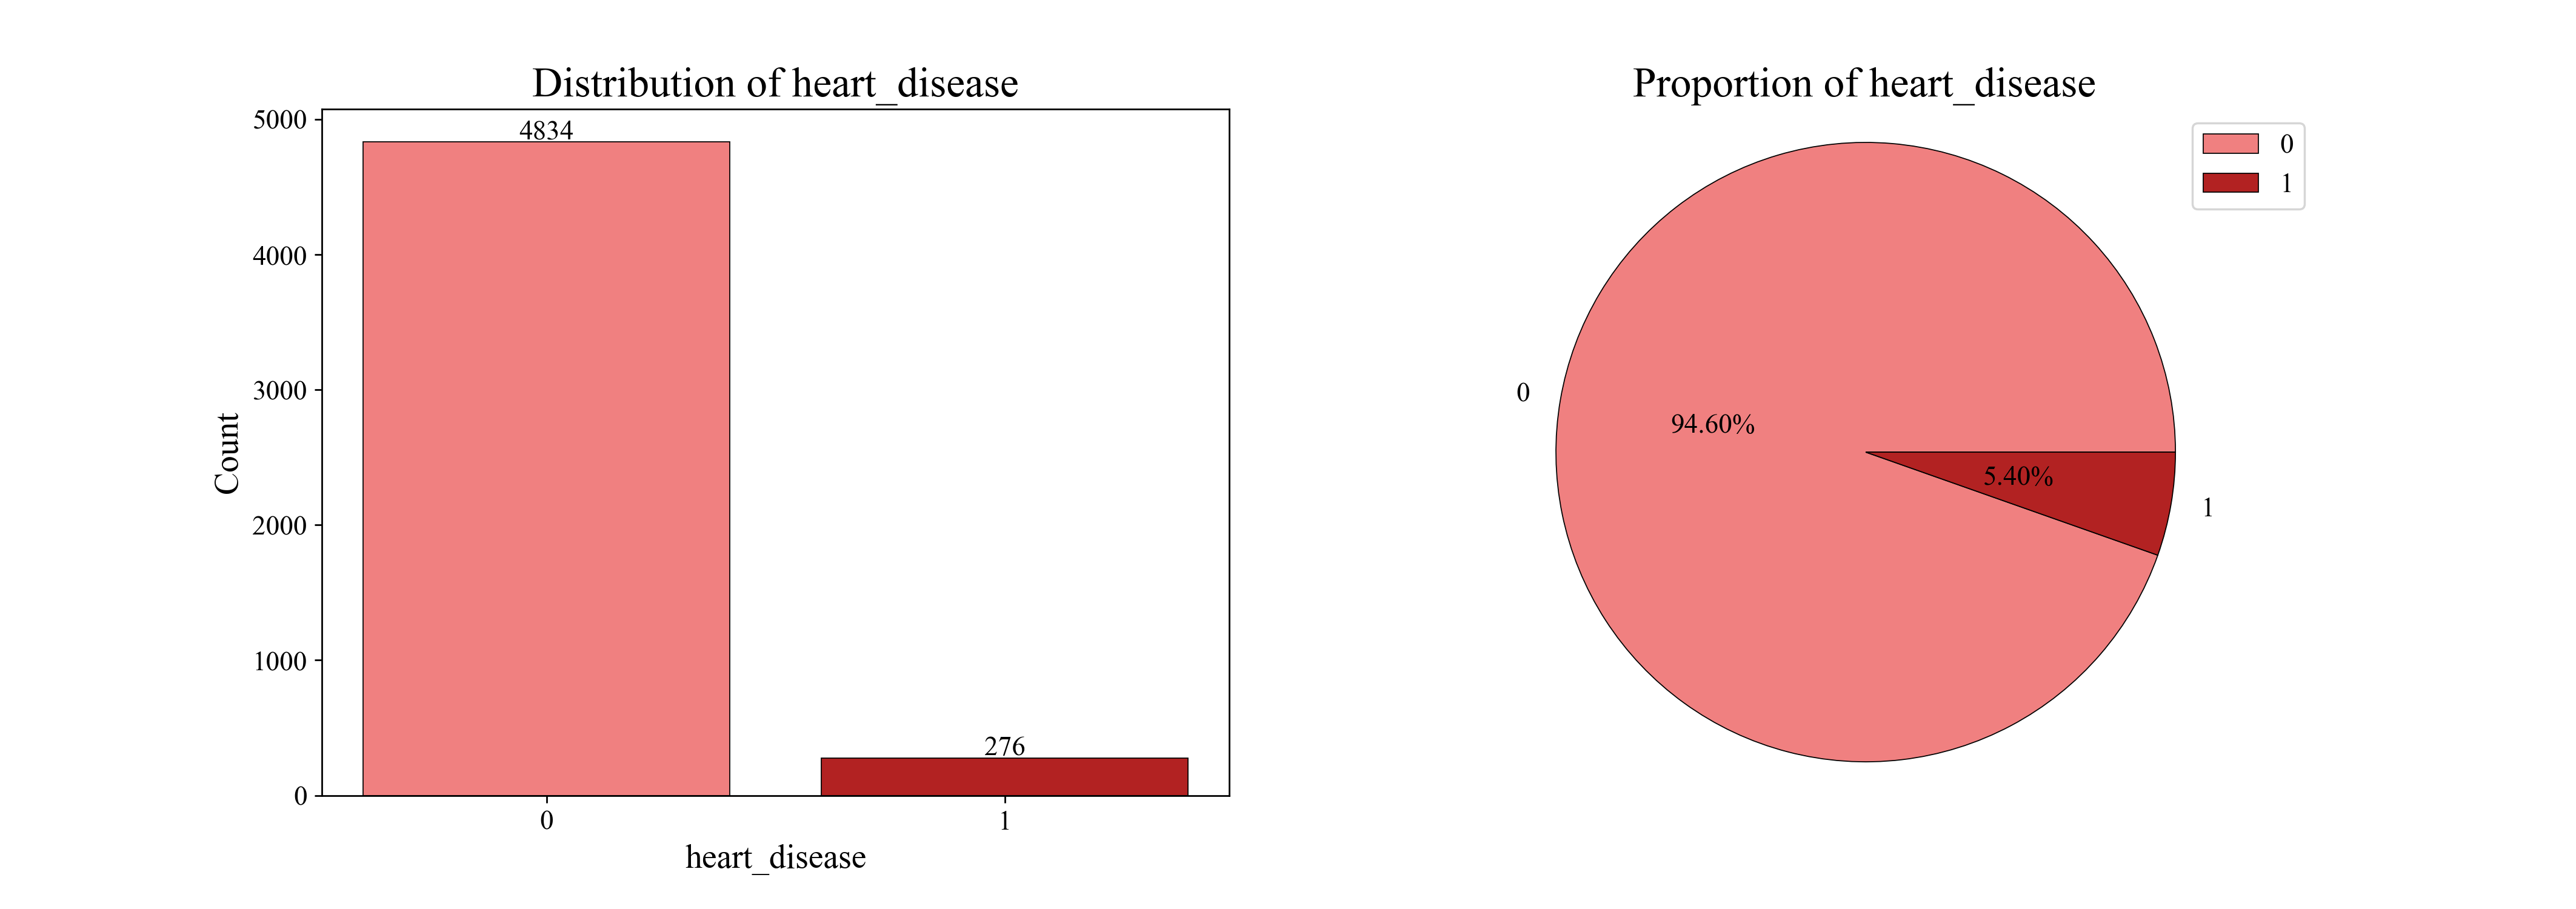
\includegraphics[width=13.5cm]{./images/heartd_bar_pie.png}

\subsection{Ever married}
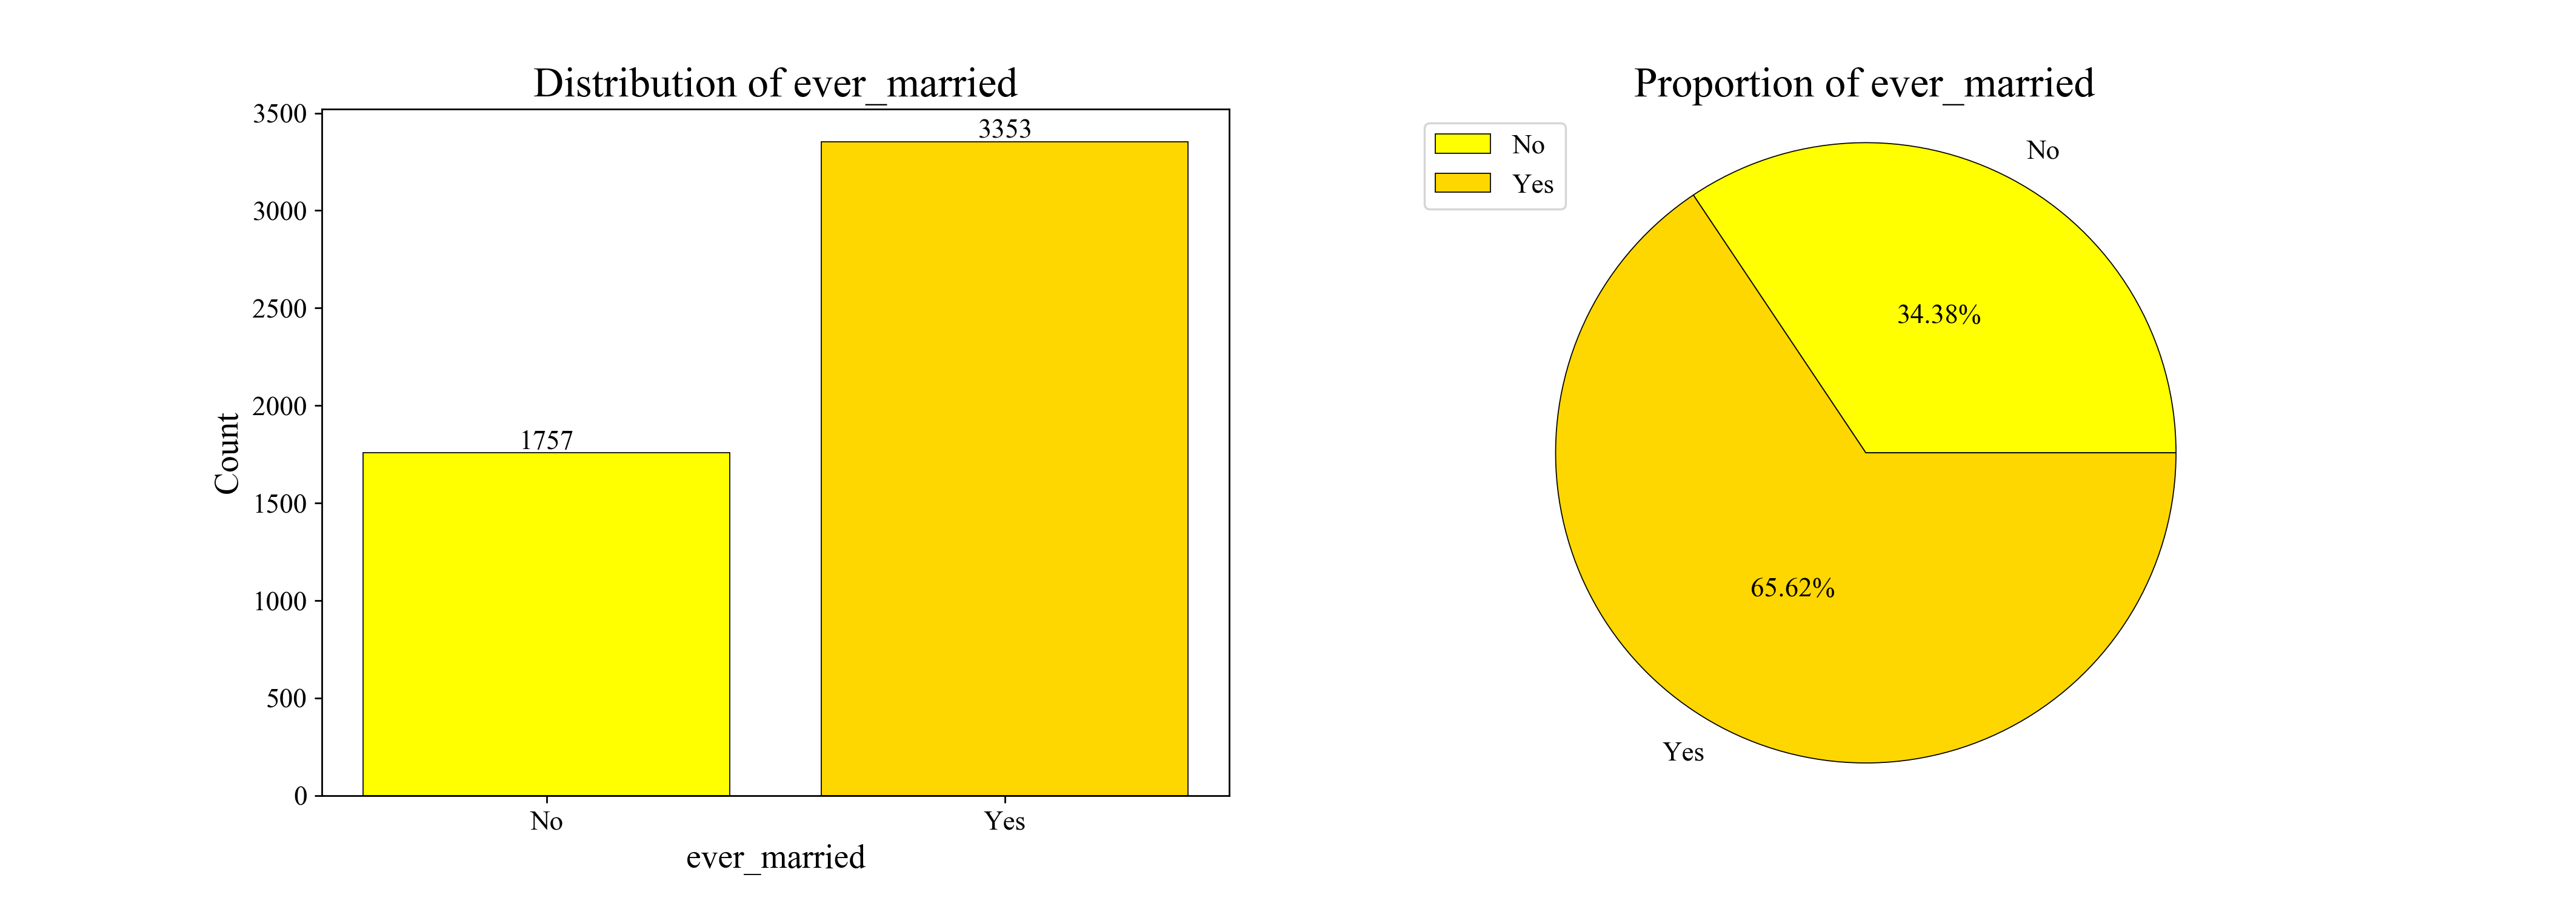
\includegraphics[width=13.5cm]{./images/evermarry_bar_pie.png}

\subsection{Residence type}
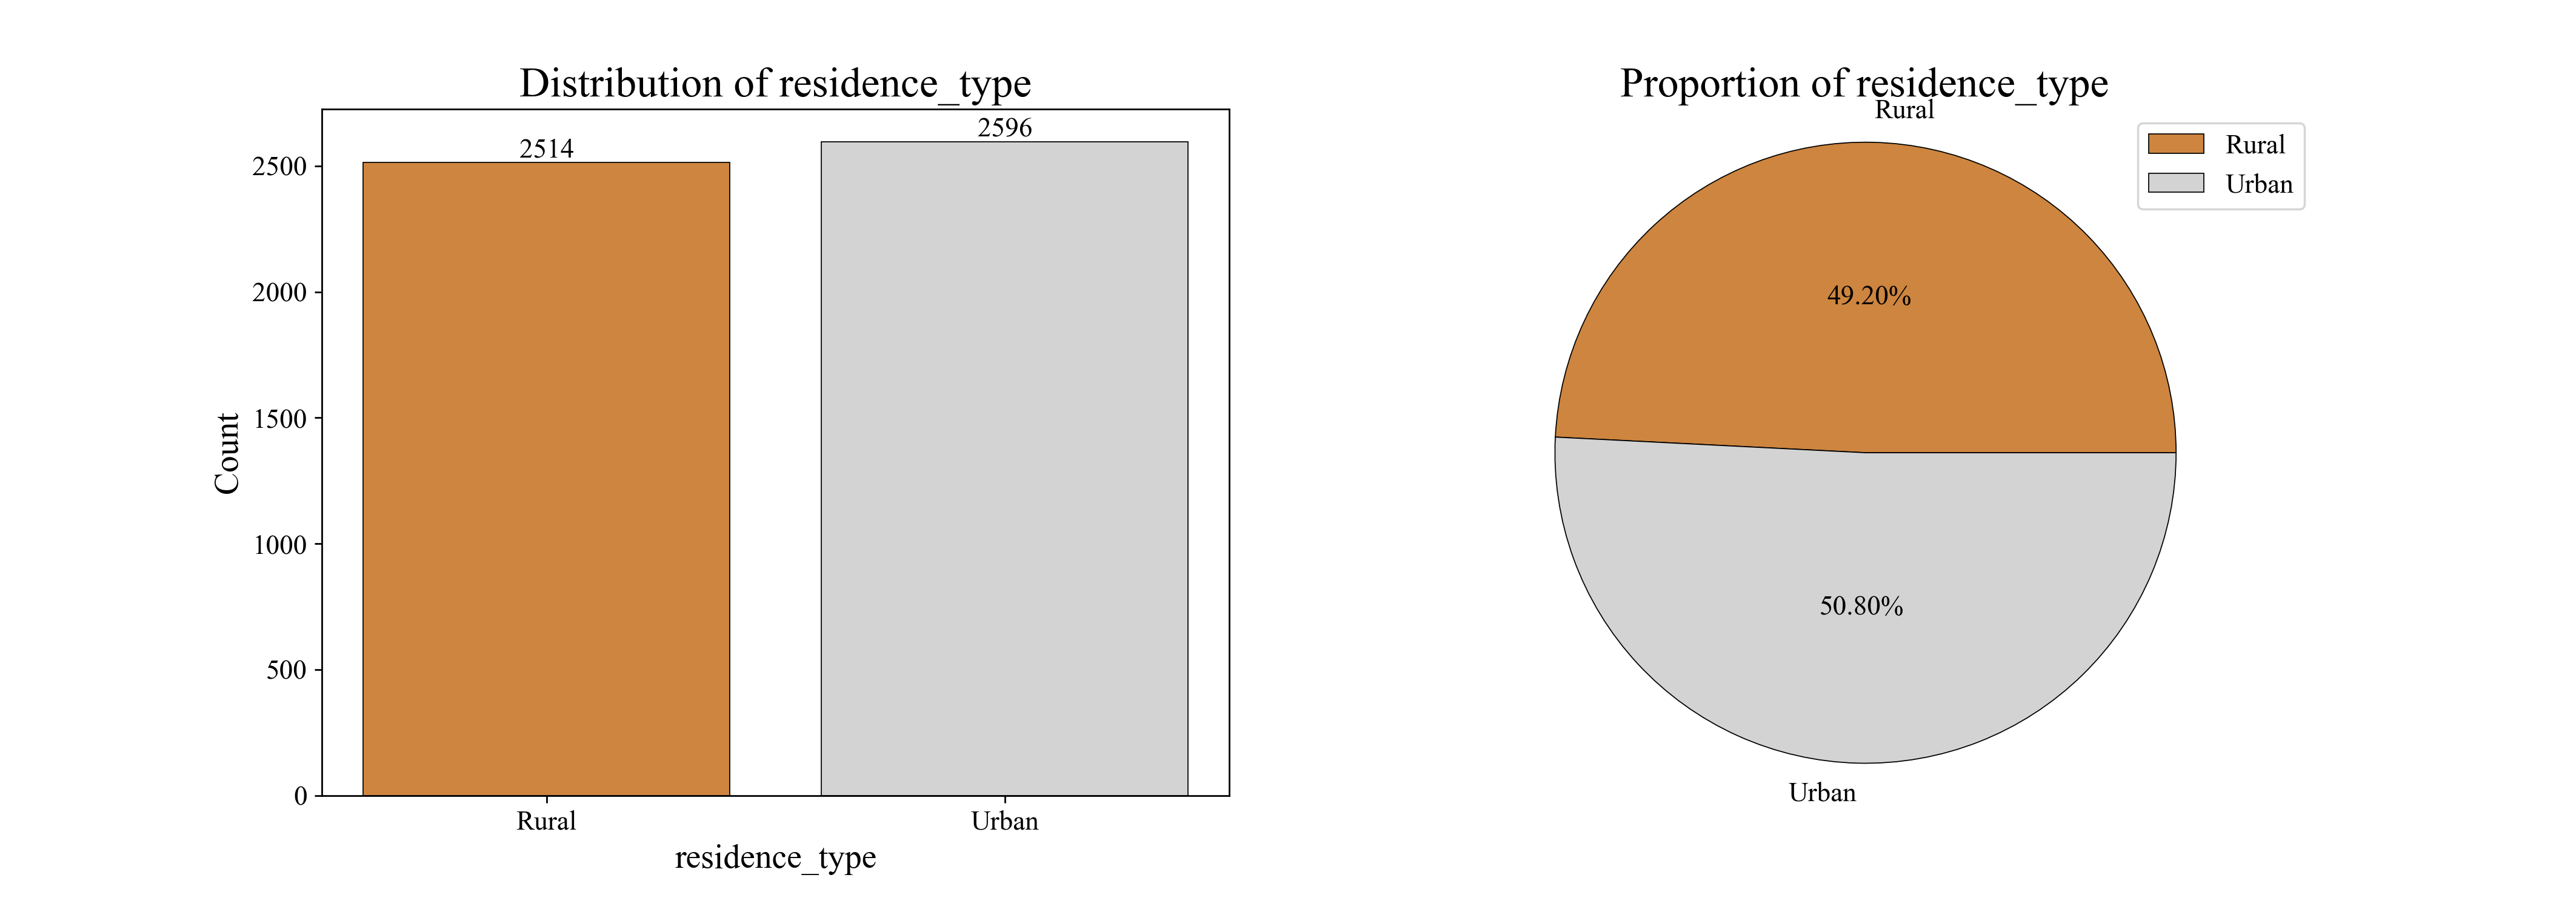
\includegraphics[width=13.5cm]{./images/resit_bar_chart.png}

\subsection{Stroke}
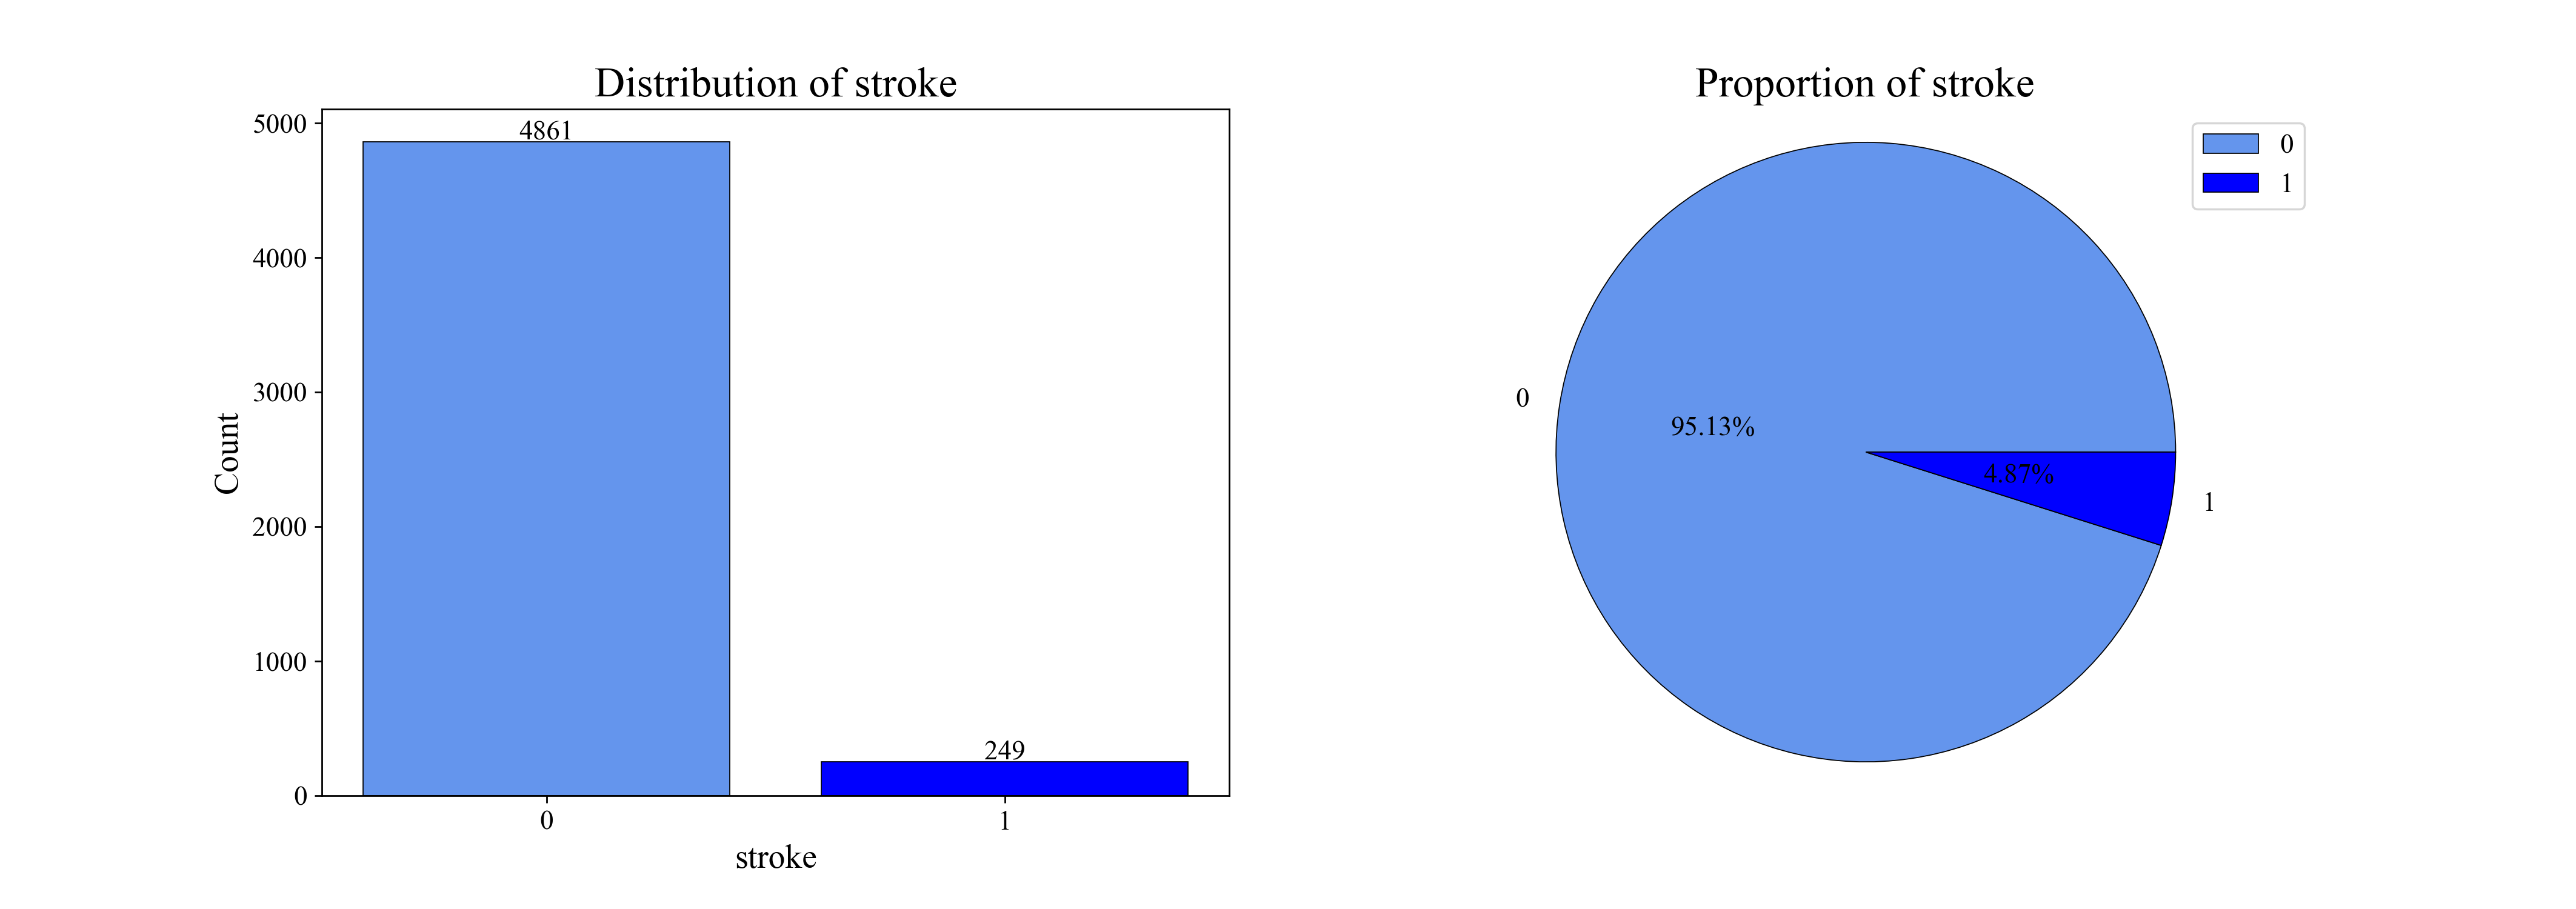
\includegraphics[width=13.5cm]{./images/stroke_bar_pie.png}

\subsection{Smoking status}
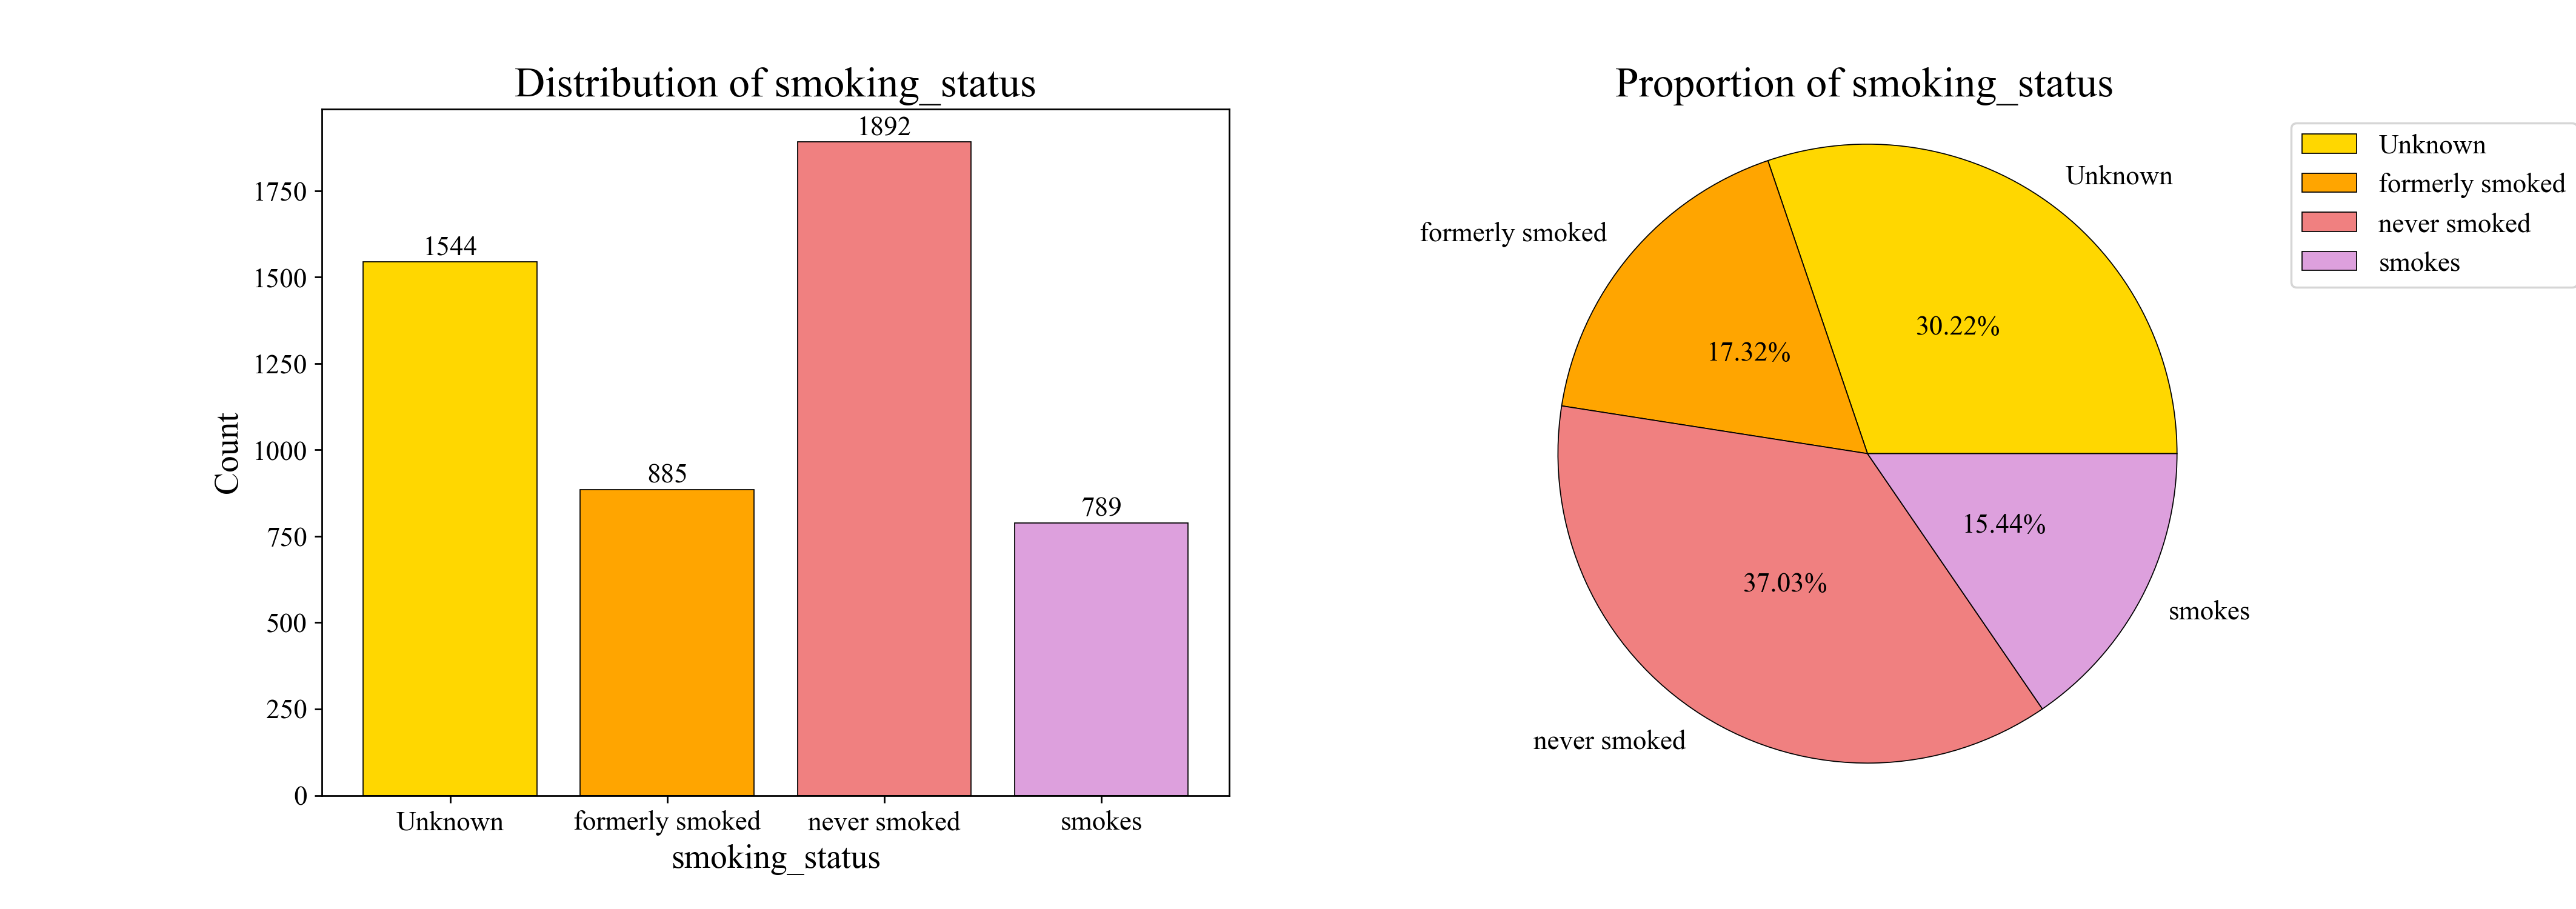
\includegraphics[width=13.5cm]{./images/smoking_bar_pie.png}

\subsection{Work type}
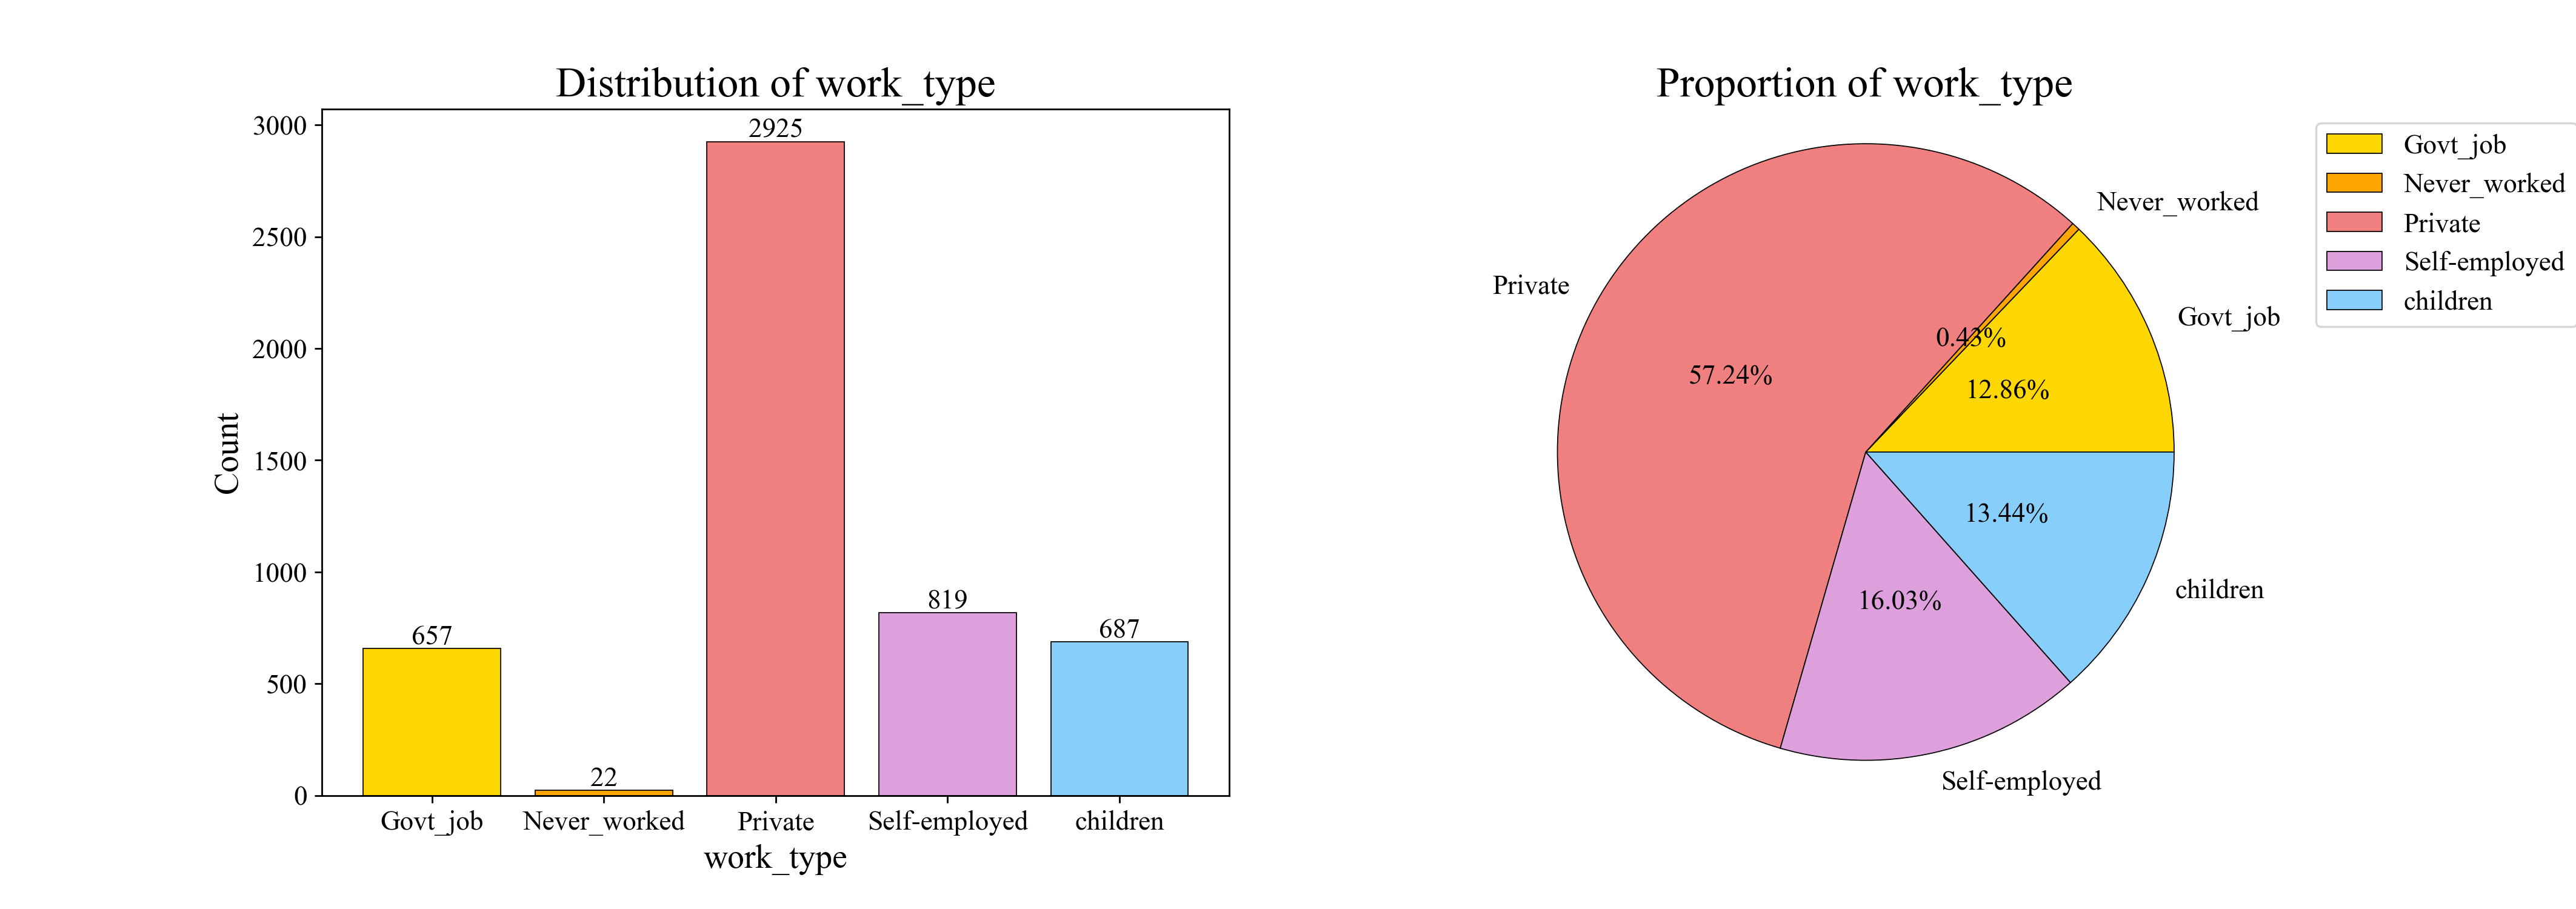
\includegraphics[width=13.5cm]{./images/worktype_bar_pie.png}

\section{單變數分析: 數值型}
\subsection{age}
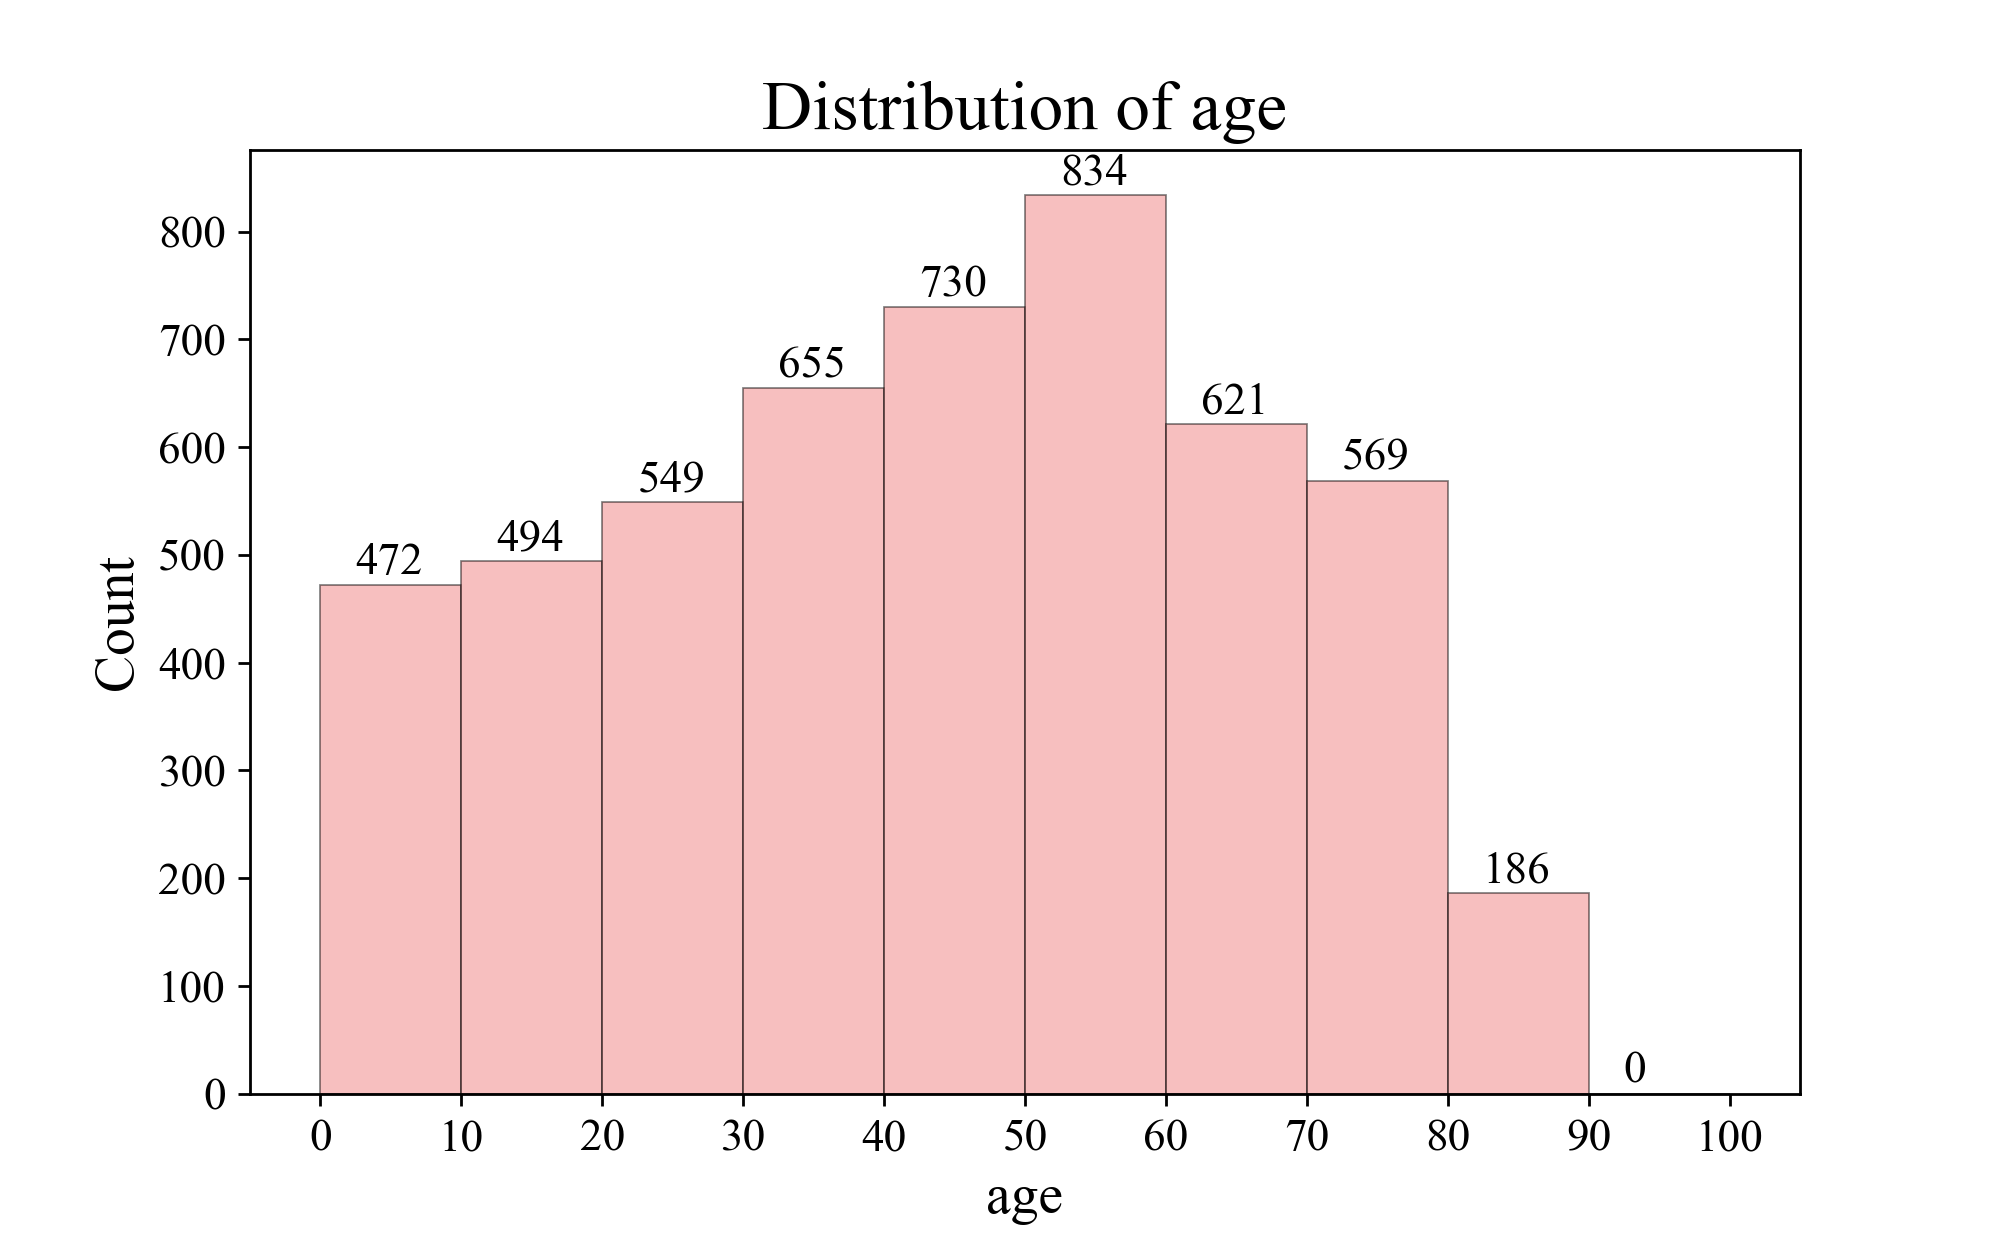
\includegraphics[height=7cm]{./images/age_distribution.png}

\subsection{Average glucose level}
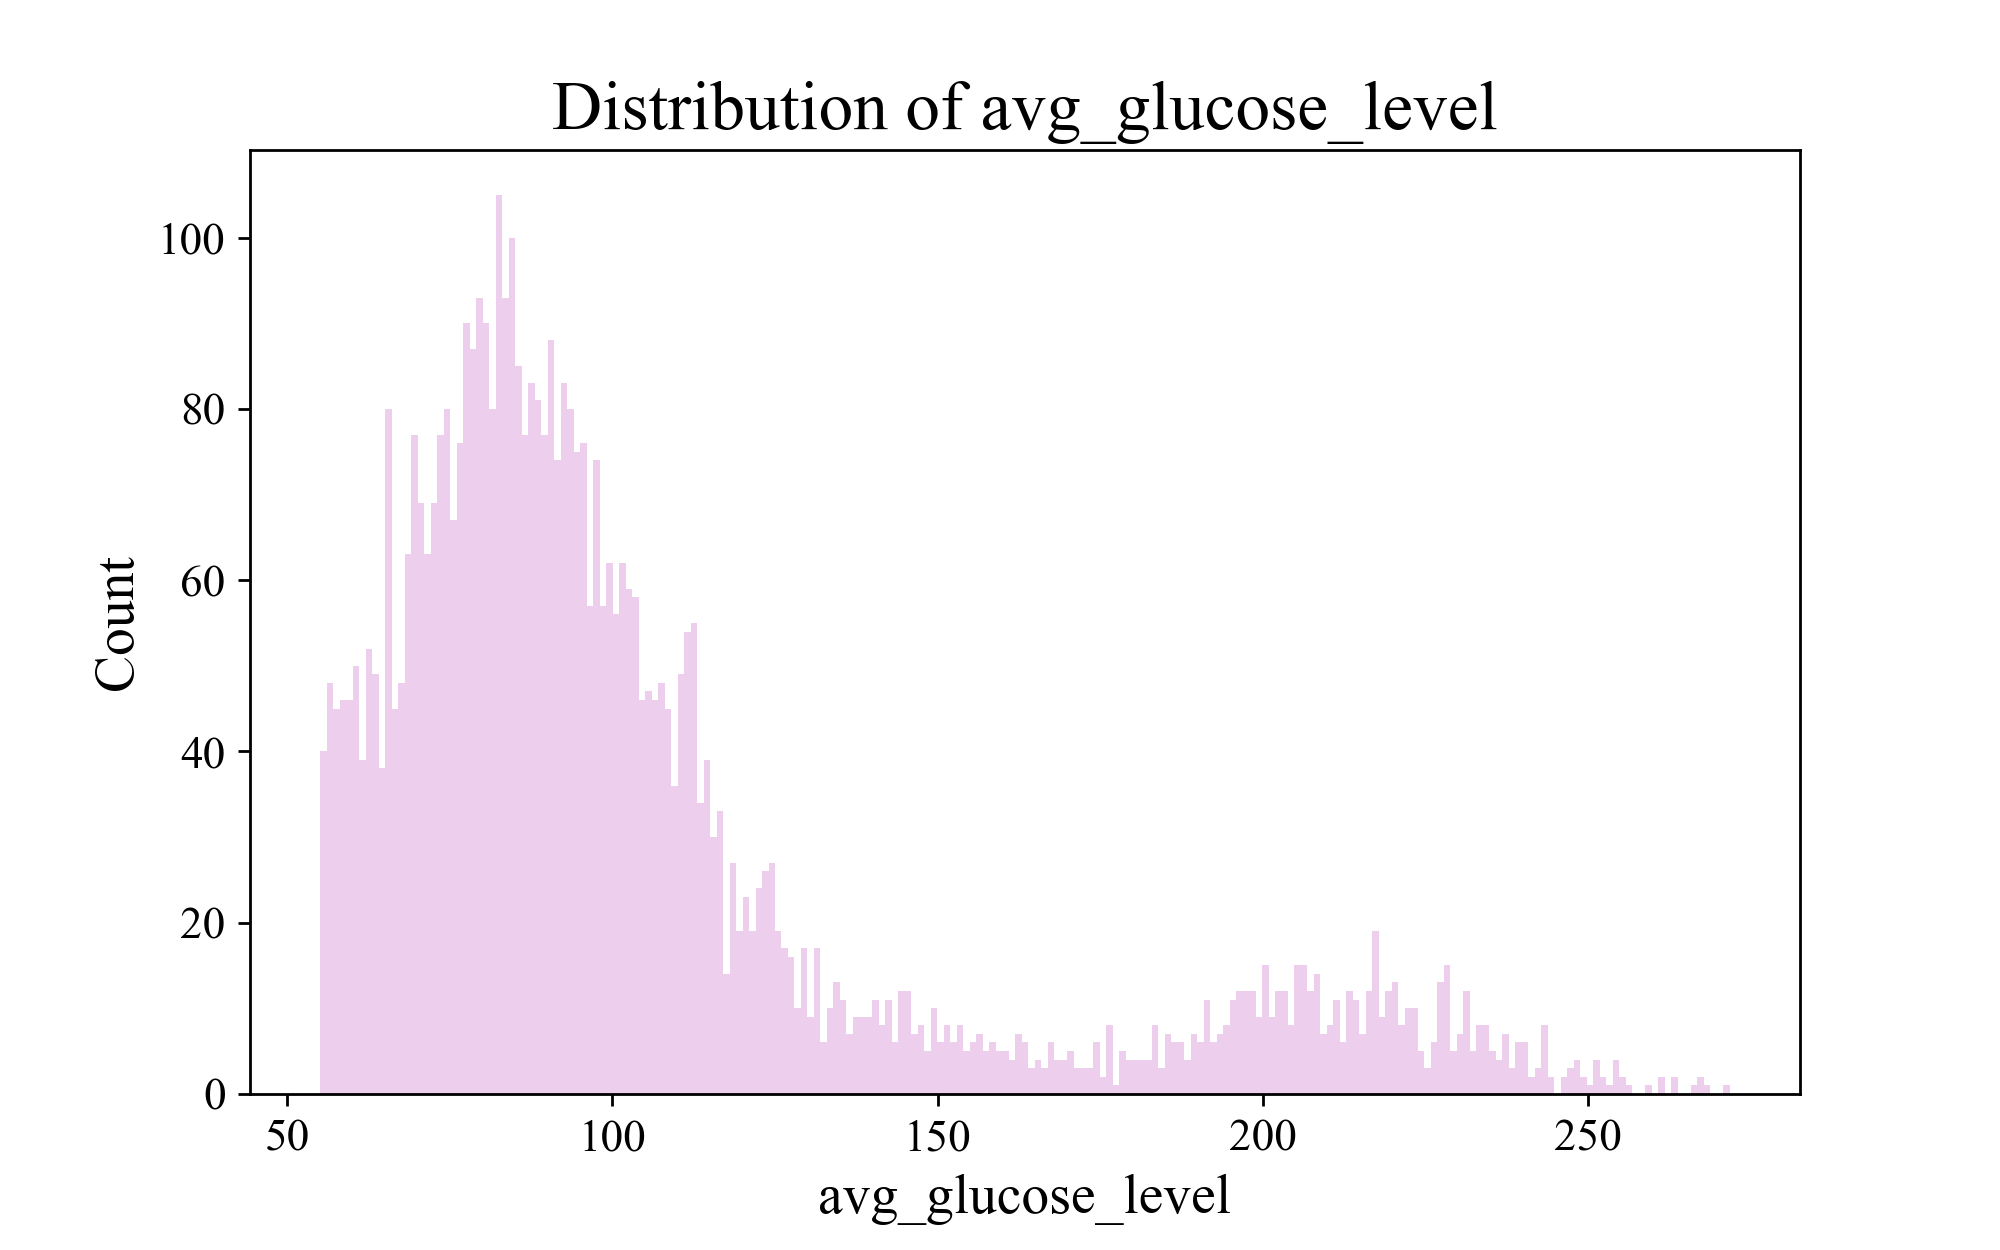
\includegraphics[height=7cm]{./images/avg_glucose_distribution.png}

\subsection{BMI}
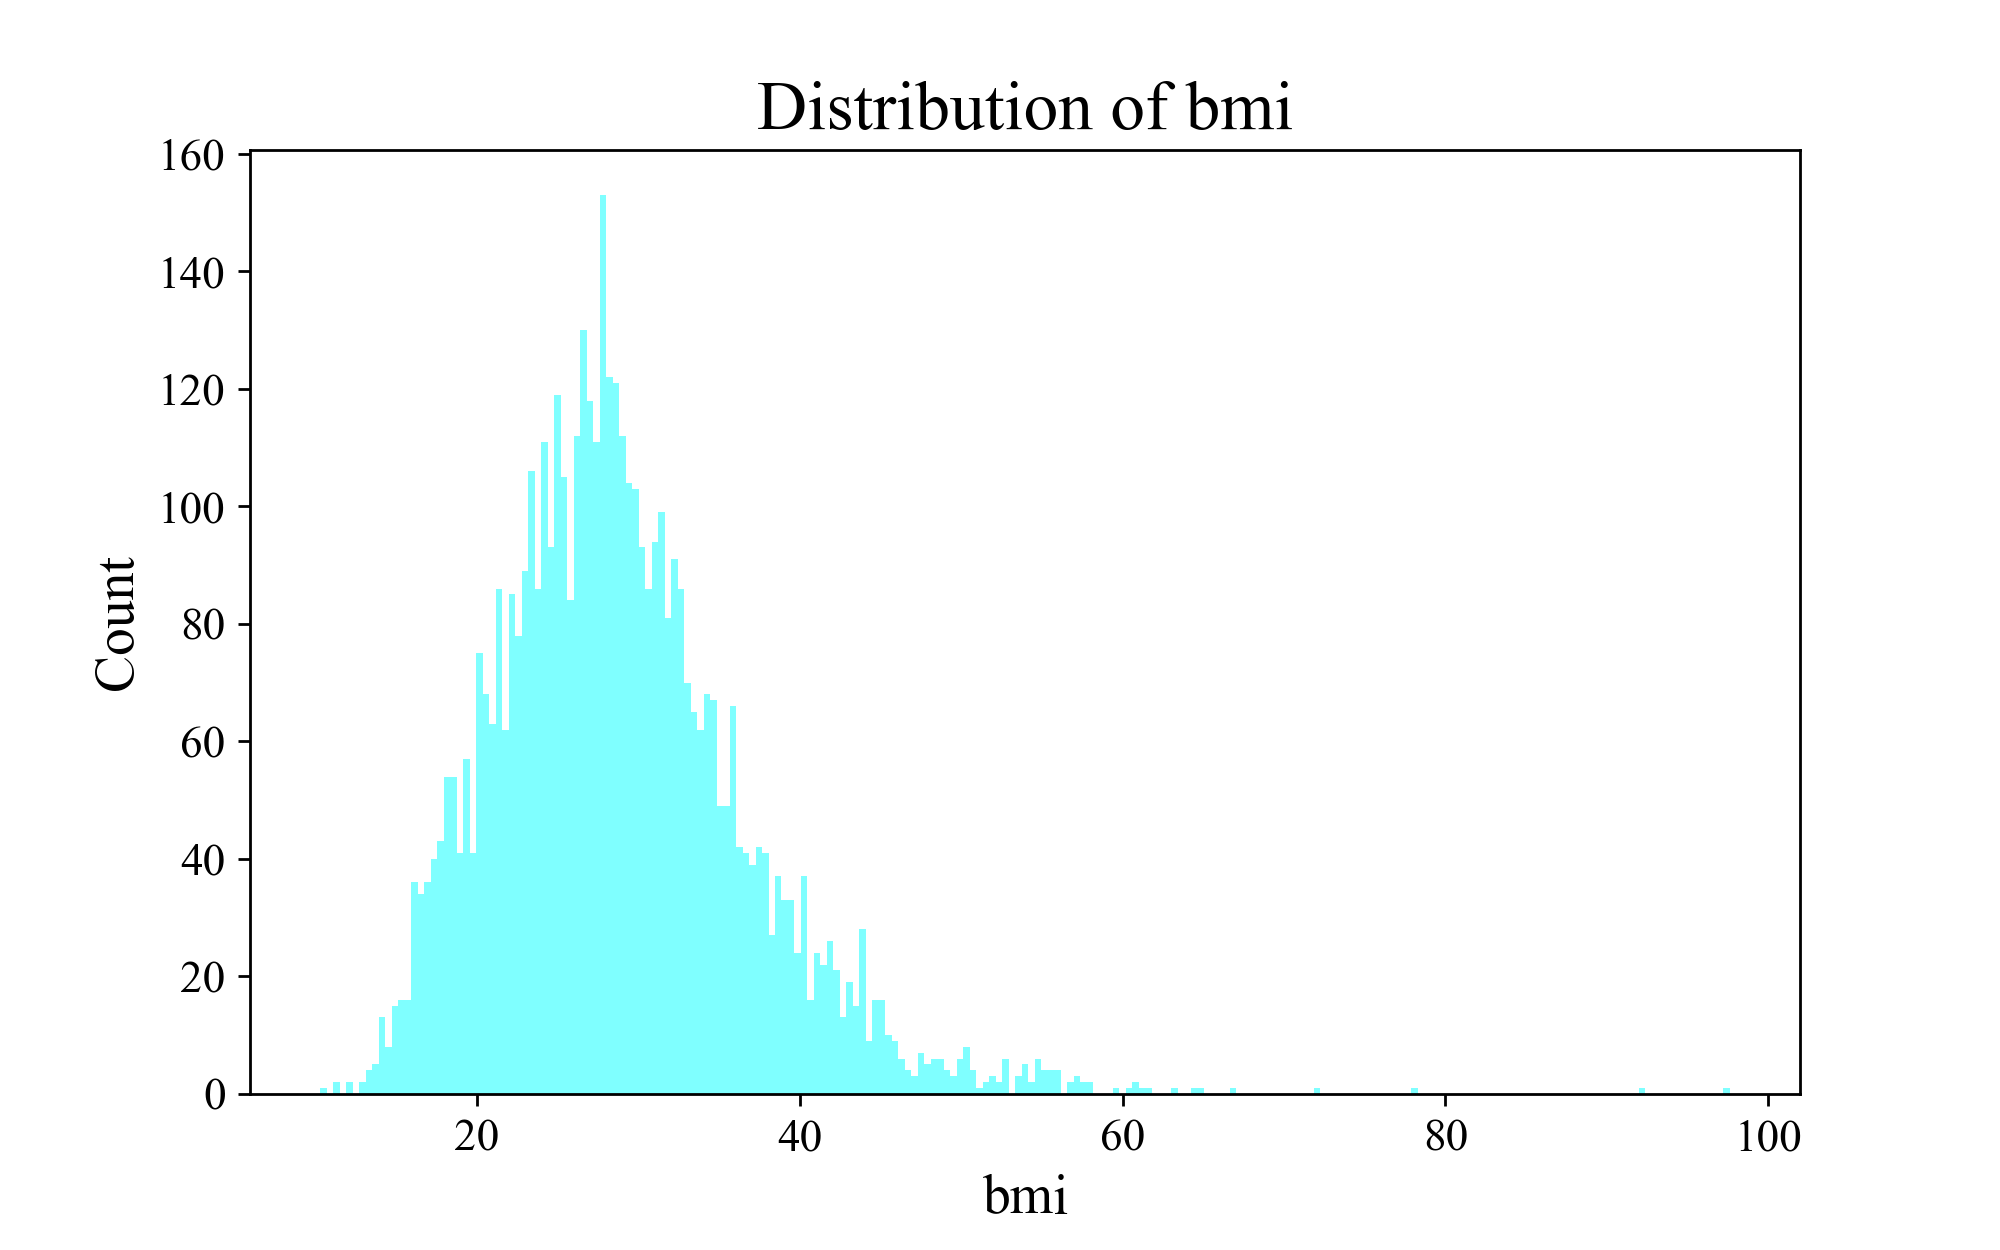
\includegraphics[height=7cm]{./images/bmi_distribution.png}



